\documentclass[aspectratio=169]{beamer}              % only frames

% for themes, etc.
\mode<presentation>
\usetheme{Madrid} 
\usecolortheme{crane}

%\usepackage{times}  % fonts are up to you
% The usual suspects
\usepackage{multirow, booktabs, dcolumn, color, graphicx} % Tables\usepackage{graphicx}
\usepackage{amsmath,amssymb,amsthm}
% Strikethrough text
\usepackage{soul}
% Adjust box to fit tabulars
\usepackage{adjustbox}
% Embed video
\usepackage{media9}
% For notes
\usepackage{pgfpages}
\setbeameroption{hide notes} % Only slides
%\setbeameroption{show only notes} % Only notes
%\setbeameroption{show notes on second screen=right} % Both
% Give a slight yellow tint to the notes page
%\setbeamertemplate{note page}{\pagecolor{yellow!5}\insertnote}\usepackage{palatino}
% Use colors by name
\usepackage{xcolor}
% EMBEDDING VIDEO IS POSSIBLE WITH PDFPC USE PDF PC to present
\usepackage{multimedia}



% The table highlighting for hypothesis discussion.
\usepackage[beamer,customcolors]{hf-tikz}
\usetikzlibrary{calc}

% To use background images
\newenvironment{colorframe}[2][]{%
\setbeamercolor{background canvas}{bg=#1}
\begin{frame}\color{white}}
{\end{frame}}


% To set the hypothesis highlighting boxes red.
\tikzset{hl/.style={
    set fill color=red!80!black!40,
    set border color=red!80!black,
  },
}

% Set Graphics folder
\graphicspath{{./figures/}}


% these will be used later in the title page
\title{Leaving Traces Online}
\subtitle{Securing Yourself in the Modern World}
\author{Irfan Kanat}
\institute[CBS]{{Department of Digitization}\\ Copenhagen Business School}
\date{\today}



\begin{document}

% this prints title, author etc. info from above
\begin{frame}

	\titlepage

	\vfill
	{\tiny \centering This work is licensed under a \href{http://creativecommons.org/licenses/by/4.0/}{Creative Commons Attribution 4.0 International License}.}

\end{frame}

\note{In this module we will talk about what kind of traces we leave going about our daily lives and how to minimize this.}

\begin{frame}
	\frametitle{Cat Video Here}
    

\end{frame}

\begin{frame}
	\frametitle{How Internet Works?}
    
    \movie{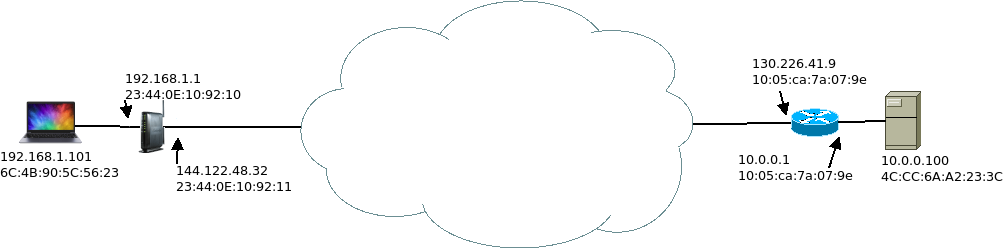
\includegraphics[width = \textwidth]{figures/RoutingA.png}}{figures/Routing.mp4}

\end{frame}

\note{For most of us Internet just works, we don't have to think about it. Understanding it a bit better on the other hand may allow us to realize what kinds of threats we may be facing. So let us start by talking about the infrastructure that makes this happen.

When you click on that link that says Cute Cat, your computer makes a request to the server computer that holds the cute cat video. This request is handed to your wifi router at home that is connected to your ISP (TDC, Waoo, etc.). From there the request is handed from one company's routers to the next, much like a bucket brigade, until it reaches the server hosting the video. Then the server sends back the file you requested the same way, from one router to the next.}

\begin{frame}
	\frametitle{Your Actions Echo Through Eternity}
    
    \centering
    
    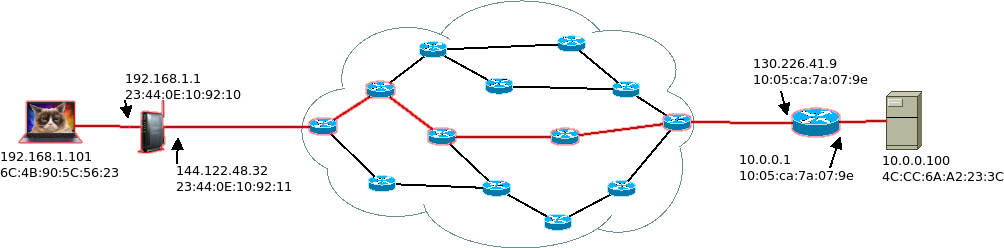
\includegraphics[width = \textwidth, height = .85\textheight, keepaspectratio]{figures/RoutingPath.png}

\end{frame}

\note{You need to realize, you leave traces of your activity along every device the packages pass through. 

This is even more sobering, considering that the routers along the way are operated by many different companies and groups that have their own interests.}

\begin{frame}
	\frametitle{Every Device Along the Way is a Possible Weakness}
    
    
\movie{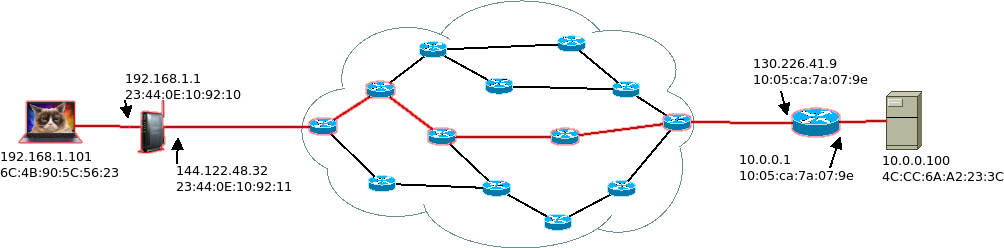
\includegraphics[width = \textwidth]{figures/RoutingPath.png}}{figures/YesThoseToo.mp4}

\end{frame}

\note{Now let us talk about some of these devices and some of the traces you leave, as well as how to minimize your footprint to make tracking harder.

Note that this is not an exhaustive list, as possible different combinations of software/hardware/connection types makes creating an exhaustive list quite hard.

\tiny{This video uses creative commons licensed sound effects from Mark DiAngelo.}}

\begin{frame}
	\frametitle{Your Device}
    
	    \begin{columns}
			\begin{column}{0.5\textwidth}
	
			It may be your computer, laptop, or cellphone...

				\begin{itemize}
					\item Browsing History
					\item Cookies from the websites
					\item Your Network addresses (MAC and IP)
					\item Configuration of your system...
				\end{itemize}	
		
			\end{column}
	
			\begin{column}{0.5\textwidth}
	
				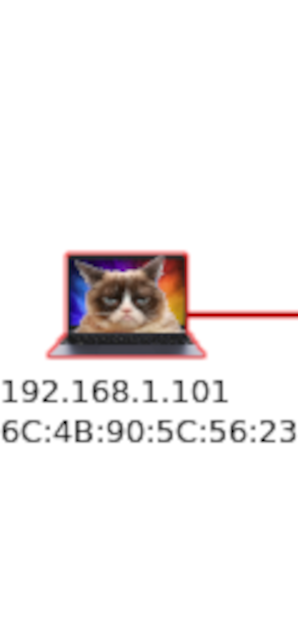
\includegraphics[width = \textwidth, height = .85\textheight, keepaspectratio]{figures/YourDevice.png}
	
			\end{column}
	
		\end{columns}

\end{frame}

\note{When you browse to a web site, your browser creates a request for that web site and sends it to your router. Then it displays the response from the other side on your computer. This leaves valuable pieces of information on your system.

Your browser keeps records of your browsing history.

Temporary files stored on your system (e.g. images on that web site can be stored in cache).

If you saved your password in your browser, it can be retrieved.

Beyond that, the websites you visit also install small files called cookies.

Depending on how it is done, when you visit a web site, the device can also reveal some details of your configuration (fonts installed, screen resolution, network addresses, etc.). These tidbits can be used to uniquely fingerprint your specific device.}

\begin{frame}
	\frametitle{What Can Be Done About Your Device?}
    
	    \begin{columns}
			\begin{column}{0.5\textwidth}
	
				\begin{itemize}
					\item USE A STRONG PASSWORD
					\item Update your software
					\item Delete Browsing History
					\item Disallow Cookies
					\item Don't Save Passwords in Browser
					\item Use Private Browsing
				\end{itemize}	
		
			\end{column}
	
			\begin{column}{0.5\textwidth}
	
				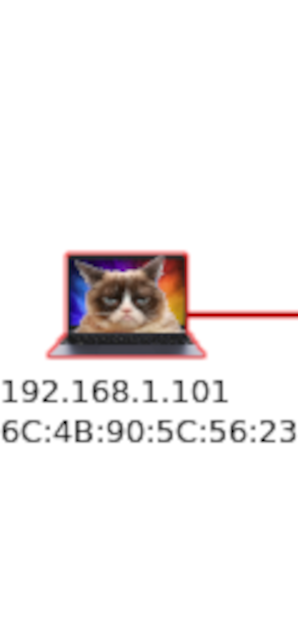
\includegraphics[width = \textwidth, height = .85\textheight, keepaspectratio]{figures/YourDevice.png}
	
			\end{column}
	
		\end{columns}

\end{frame}

\note{If you don't want someone with access to your device to discover your activities, here is what you can do:

USE A STRONG PASSWORD ON YOUR DEVICE. Limit physical access. This is sensible because anyone that gains access to your operating system can gain access to way more than what we discuss below.

You can delete the browser history, and cookies.

If you don't want the web site you are visiting to be able to install permanent cookies on your machine, or leave traces of your visit on your computer. You can use private browsing.

Note that neither of these solutions will prevent someone that has access to your wi-fi router to reconstruct your browsing history. So while these precautions may prevent your room mate from discovering your Star Wars fan-fic addiction that goes on into late in the night, it won't prevent your ISP.

If you are getting your internet access through your work, then your boss may also know about your guilty pleasure of reading steamy Kylo Ren, Rey, Chewbacca love triangle stories.}

\begin{frame}
	\frametitle{Your Router}
    
    	\begin{columns}
			\begin{column}{0.5\textwidth}
	
			This is the device you host on your premises.

				\begin{itemize}
					\item Every Package You Send/Receive
					\item DNS querries
					\item Your and Target Servers' IP addresses
					\item ISP shenanigans...
				\end{itemize}	
		
		\end{column}
	
		\begin{column}{0.5\textwidth}
	
				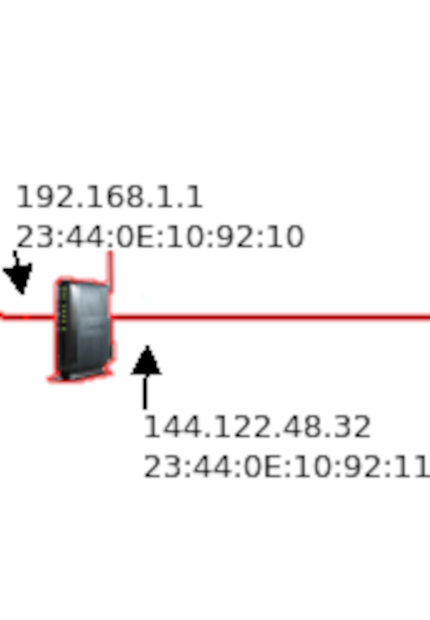
\includegraphics[width = \textwidth, height = .85\textheight, keepaspectratio]{figures/YourRouter.png}
	
		\end{column}
	
		\end{columns}

\end{frame}

\note{Most times you simply call it Wi-Fi. You have physical access to it, but in some cases (cable internet) your ISP may administer it. It is a small box, connected to either phone/cable/fiber optic cables. Who ever has control of this device has access to all the traffic going through it. Typically, you and your ISP have access to this traffic. Malicious actors may also gain access to these devices.

When you write a url in your browser (like www.google.com) it sends a query to an addressing system to match that url to a network address. These DNS queries go unencrypted (although it is changing nowadays). That means, just by looking at your DNS querries, someone may figure out which websites you visit.

The messages sent between you and the otherside go through this device. In the past, most web traffic was unencrypted. That meant they could read every message passing through. These days, most web traffic is encrypted. This means they can't directly read your messages (unless they also do a TLS intercept). Still the volume, timing, and destination of traffic tells them quite a lot. 

In certain cases, they may play a sort of man-in-the-middle attack to decrypt your encrypted traffic (TLS intercept).

In US in the past, ISPs have been known to add tracking identifiers to certain packages to sell advertising data.
}

\begin{frame}
	\frametitle{What Can Be Done About Your Router?}
    
     	\begin{columns}
			\begin{column}{0.5\textwidth}
	
			This is the device you host on your premises.

				\begin{itemize}
					\item Use Encrypted Protocols
					\item Keep the Device Updated
					\item Use Strong Passwords
					\item Disable Remote Administration
				\end{itemize}	
		
		\end{column}
	
		\begin{column}{0.5\textwidth}
	
				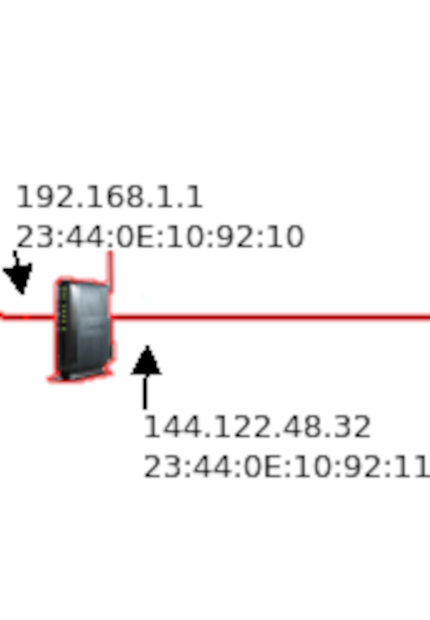
\includegraphics[width = \textwidth, height = .85\textheight, keepaspectratio]{figures/YourRouter.png}
	
		\end{column}
	
		\end{columns}   

\end{frame}

\note{Whenever you can use encrypted protocols. HTTPs is already wide spread. Use DNScrypt to encrypt your DNS traffic.

Make sure your router is receiving latest firmware updates. The device manifacturers stop releasing updates so many years after release, don't use devices that are not receiving regular updates.

Use strong passwords to prevent outside parties from gaining access to your hardware. Disable remote administration of your hardware also.

Even after doing all this your traffic meta-data will still be accessible to people who have access to your router. This means they will know which servers you communicated, when you communicated, and the volume of the traffic.
}

\begin{frame}
	\frametitle{Other Routers}
    
        \begin{columns}
    		\begin{column}{0.5\textwidth}
    
    			Controlled by others.

    			\begin{itemize}
					\item Every Package You Send/Receive
					\item DNS querries
					\item Your and Target Servers' IP addresses
				\end{itemize}	
    	
    		\end{column}
    
    		\begin{column}{0.5\textwidth}
    
    			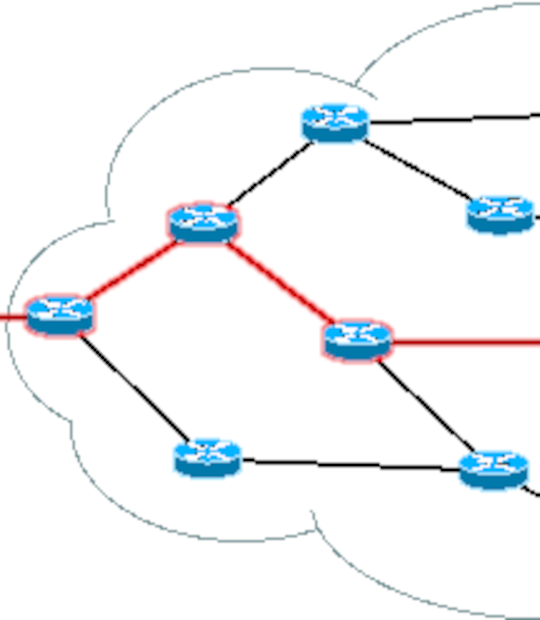
\includegraphics[width = \textwidth, height = .85\textheight, keepaspectratio]{figures/OtherRouters.png}
    
    		\end{column}
    
    	\end{columns}

\end{frame}

\note{Wild thing about the internet is, your traffic goes through many different devices, controlled by many different organizations. The information at risk is much the same as your own router, except your control over the situation is even less.

The people who operate the routers have access to all traffic going through.

Movie industry has forced some ISP's in certain countries in the past to reveal customer information to target for piracy litigation.

Typically, first router after your own is operated by your ISP. In US NSA, and in UK GHCQ are known to be tapped directly into ISP networks to siphon off all the traffic.

The routers can be tricked into redirecting traffic into certain routers. China is known to siphon off European traffic this way from time to time.}

\begin{frame}
	\frametitle{Trace Route Demo}
    

\end{frame}

\begin{frame}
	\frametitle{What Can Be Done About Other Routers}
    
        \begin{columns}
    		\begin{column}{0.5\textwidth}
    
    			Who are you worried about?

    			\begin{itemize}
					\item VPN
					\item TOR Network
				\end{itemize}	
    	
    		\end{column}
    
    		\begin{column}{0.5\textwidth}
    
    			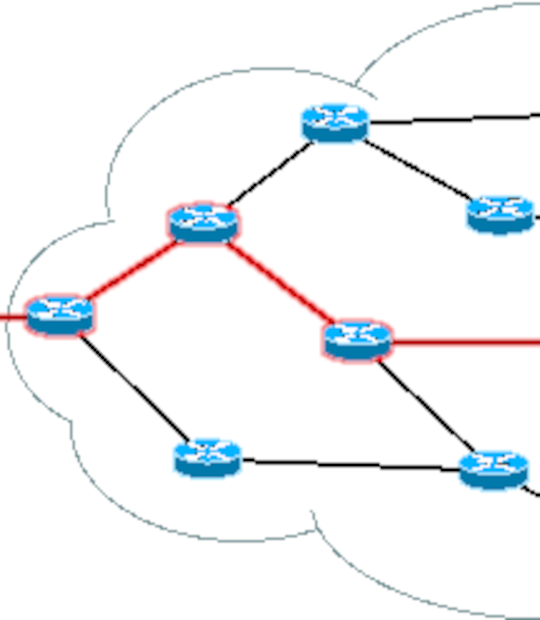
\includegraphics[width = \textwidth, height = .85\textheight, keepaspectratio]{figures/OtherRouters.png}
    
    		\end{column}
    
    	\end{columns}

\end{frame}

\note{
	If you are worried about private third parties violating your privacy (e.g. Lawyers working for Film and Music industry), you can use a VPN.

	This means you send all your packages to a VPN server over an encrypted link, and the VPN server will make your requests for you. That way, your traffic can not be linked to you. Most VPN operators also allow you to chose the exit nodes. This allows you to bypass geographic limitations such as certain movies being only visible to American Netflix Users, or BBC broadcast being only available in the UK. 

	The government can suponea the VPN operator to access traffic data. It is wise to pick a VPN operator that is based in countries with tighter privacy laws. You also probably wouldn't want a VPN from a country that has intelligence sharing agreements with US (See five-eyes, nine-eyes, 14 eyes). Read more about it here: https://opennet.net/research/regions/nordic-countries

	If you are worried about Nation State Actors monitoring your traffic, you can consider TOR anonymizing network. It is like a VPN, except it also has a shuffling server in between the entrance and multiple possible exit nodes. The encrypted packages enter a node of the TOR network get randomly shuffled within the network and reach different end nodes before being sent to your destination server. This makes tracing traffic very hard. TOR is a favorite of criminal groups world wide. Yet in the past Intelligence agencies have found ways of compromising the TOR network. So even TOR is no guarantee against a dedicated government effort.
}

\begin{frame}
	\frametitle{VPN Demo}
    

\end{frame}

\begin{frame}
	\frametitle{The Target Server}
    
        \begin{columns}
    		\begin{column}{0.5\textwidth}
    
    			\begin{itemize}
    				\item Your IP address
    				\item What you received
    				\item What you sent
    				\item Account Information
    				\item Payment Information
    			\end{itemize}
    	
    		\end{column}
    
    		\begin{column}{0.5\textwidth}
    
    			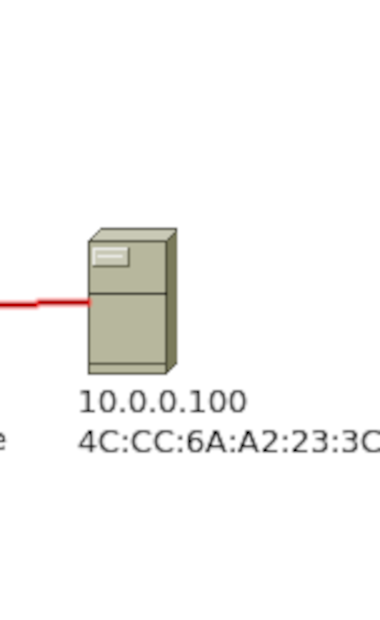
\includegraphics[width = \textwidth, height = .85\textheight, keepaspectratio]{figures/TargetServer.png}
    
    		\end{column}
    
    	\end{columns}

\end{frame}

\note{This is the device that hosted the content you interacted with. Who ever has control over this machine has access to everything you requested from it.

In the past, when governments managed to take over illegal web sites (e.g. silkroad) they let the web site operate for a period to also capture the people using the web site.}


\begin{frame}
	\frametitle{What Can Be Done About The Target Server}
    
        \begin{columns}
    		\begin{column}{0.5\textwidth}
    
    			\begin{itemize}
    				\item VPN
    				\item Limit Linkable Data
    			\end{itemize}
    	
    		\end{column}
    
    		\begin{column}{0.5\textwidth}
    
    			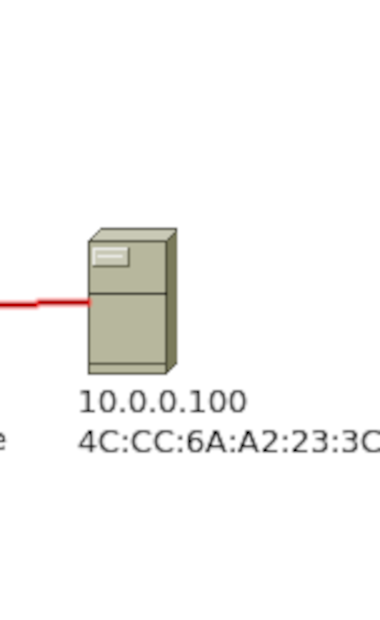
\includegraphics[width = \textwidth, height = .85\textheight, keepaspectratio]{figures/TargetServer.png}
    
    		\end{column}
    
    	\end{columns}

\end{frame}

\note{If you used any service that obfuscated your traffic (VPN, TOR) then the other side can only see the network address of the exit node and not your own address. That is already a good start.

The other piece of information the server operator has access to is the data you enter. If you entered credit card information, the credit card can already be linked to your real name and address. So if you are worried about the server operator acting maliciously, don't provide them with data that can be linked back to you (e.g. phone number, e-mail, credit card).}

\begin{frame}
	\frametitle{Threat Models}


	\centering


\adjustbox{max height=\dimexpr\textheight-5.5cm\relax,
           max width=\textwidth}{
\begin{tabular}{llll}
\textbf{Threat} &
  \begin{tabular}[c]{@{}l@{}}Ex-girlfriend/boyfriend breaking \\ into your email account and publicly\\  releasing your correspondence with\\  the My Little Pony fan club\end{tabular} &
  \begin{tabular}[c]{@{}l@{}}Organized criminals breaking\\  into your email account and \\ sending spam using your identity\end{tabular} &
  \begin{tabular}[c]{@{}l@{}}The Mossad doing Mossad\\ things with your email account\end{tabular} \\
\textbf{Solution} &
  Strong passwords &
  \begin{tabular}[c]{@{}l@{}}Strong passwords + common sense\\ (don’t click on unsolicited herbal \\ Viagra ads that result in keyloggers\\ and sorrow)\end{tabular} &
  \begin{tabular}[c]{@{}l@{}}Magical amulets?\\ \\ Fake your own death, move into a \\ submarine?\\ \\ YOU’RE STILL GONNA BE \\ MOSSAD’ED UPON\end{tabular}
	\end{tabular}}
		


	\vspace{.5em}
    \tiny(Source: James Mickens (2014) This World of Ours)

\end{frame}

\note{
	I highly recommend watching Citizen 4 about Snowden revelations. Look at how he organizes his security (encrypted communications, wiping devices, using a blanket before entering his passwords). Despite all that, he knew from the get go that he was going to get caught.

	Complete Security is not possible. We are trying to balance out security controls against adversary's capabilities and willingness to pursue us.

	The precautions you take against your mother from discovering your star wars science fiction addiction, is not the same as the precautions you take against Mette Frederiksen from discovering the same.

	So I highly recommend you take a realistic look at the threats and make an informed decision about the precautions you need to use.
}

\end{document}
